\documentclass[manuscript,review]{acmart}
\bibliographystyle{ACM-Reference-Format}
\usepackage{multirow}
\usepackage{multicol}
\usepackage{subcaption}
\title{Tackling Model Bias via Game-theoretic Multi-agent Collaboration Framework for Hateful Meme Classification}

% Use \author and \affiliation in the order that maps to the superscript numbers
\author{Yiwei Wei}
\affiliation{\institution{Tianjin Key Laboratory of Cognitive Computing and Application, Tianjin University}\country{China}}

\author{Zhengliang Guo}
\affiliation{\institution{China University of Petroleum-Beijing at Karamay}\country{China}}

\author{Shaozu Yuan}
\affiliation{\institution{Meituan}\country{China}}

\author{Chengyin Hu}
\affiliation{\institution{China University of Petroleum-Beijing at Karamay}\country{China}}

\author{Zhiyang Jia}
\affiliation{\institution{China University of Petroleum-Beijing at Karamay}\country{China}}

\author{Jiujiang Guo}
\affiliation{\institution{School of Computer Science and Technology, Tianjin University}\country{China}}

\author{Meng Chen}
\affiliation{\institution{Oracle AI}\country{Australia}}

\author{Peiying Wang}
\affiliation{\institution{Meituan}\country{China}}

\author{Longbiao Wang}
\affiliation{\institution{Tianjin Key Laboratory of Cognitive Computing and Application, Tianjin University}\country{China}}

\begin{document}
\begin{abstract}
Hateful meme classification aims to identify memes containing hateful content and has become increasingly important in the era of social media dominance. Large multimodal models (LMMs) have significantly enhanced the understanding of multimodal content, advancing this field. However, cognitive biases in LMMs can impede effective collaboration among models. To tackle this issue, we introduce \textbf{GECO}, a \textbf{G}ame-theoretic multi-ag\textbf{E}nt \textbf{C}ollaboration framewOrk that organizes multiple LMMs into interacting agents and employs game-theoretic principles to guide them toward an optimal cooperative equilibrium. GECO further integrates a mixed bonus scheme with both individual accuracy and cross-model agreement, which together drive the system toward a consistent cooperative solution. In addition, we implement efficient policy learning and introduce a penalty coefficient to optimize the framework effectively and ensure training stability. Extensive experiments on five public datasets demonstrate that our framework achieves new state-of-the-art performance. We release our code.
\end{abstract}
\maketitle
\section{Introduction}

Hateful memes are a growing problem on social media, since a single meme combines an
image and text in a way that can carry a hateful message even when neither the image
nor the text is offensive on its own. This makes automatic detection difficult, and the
problem has become more urgent as harmful content contributes to online harassment and
real-world consequences for the people targeted.

Earlier detection systems relied on pretrained vision-language models combined with a
task-specific classifier layer. More recently, large multimodal models (LMMs) have
taken over this space because of their much stronger reasoning ability over combined
image and text input. Some works try to push a single LMM further, for example by adding
LoRA-based adapters for few-shot learning, or by retrieving similar examples to help the
model decide.

The core issue is that any single LMM carries its own biases, inherited
from its training data and architecture. To reduce this, researchers have tried combining
multiple models together instead of relying on one. These multi-agent approaches
generally fall into two camps: \textbf{voting-based} methods, where multiple models each vote
and the majority decision wins, and \textbf{debate-based} methods, where models argue different
interpretations and a separate judge model decides the outcome.

\begin{figure}[h]
    \centering
    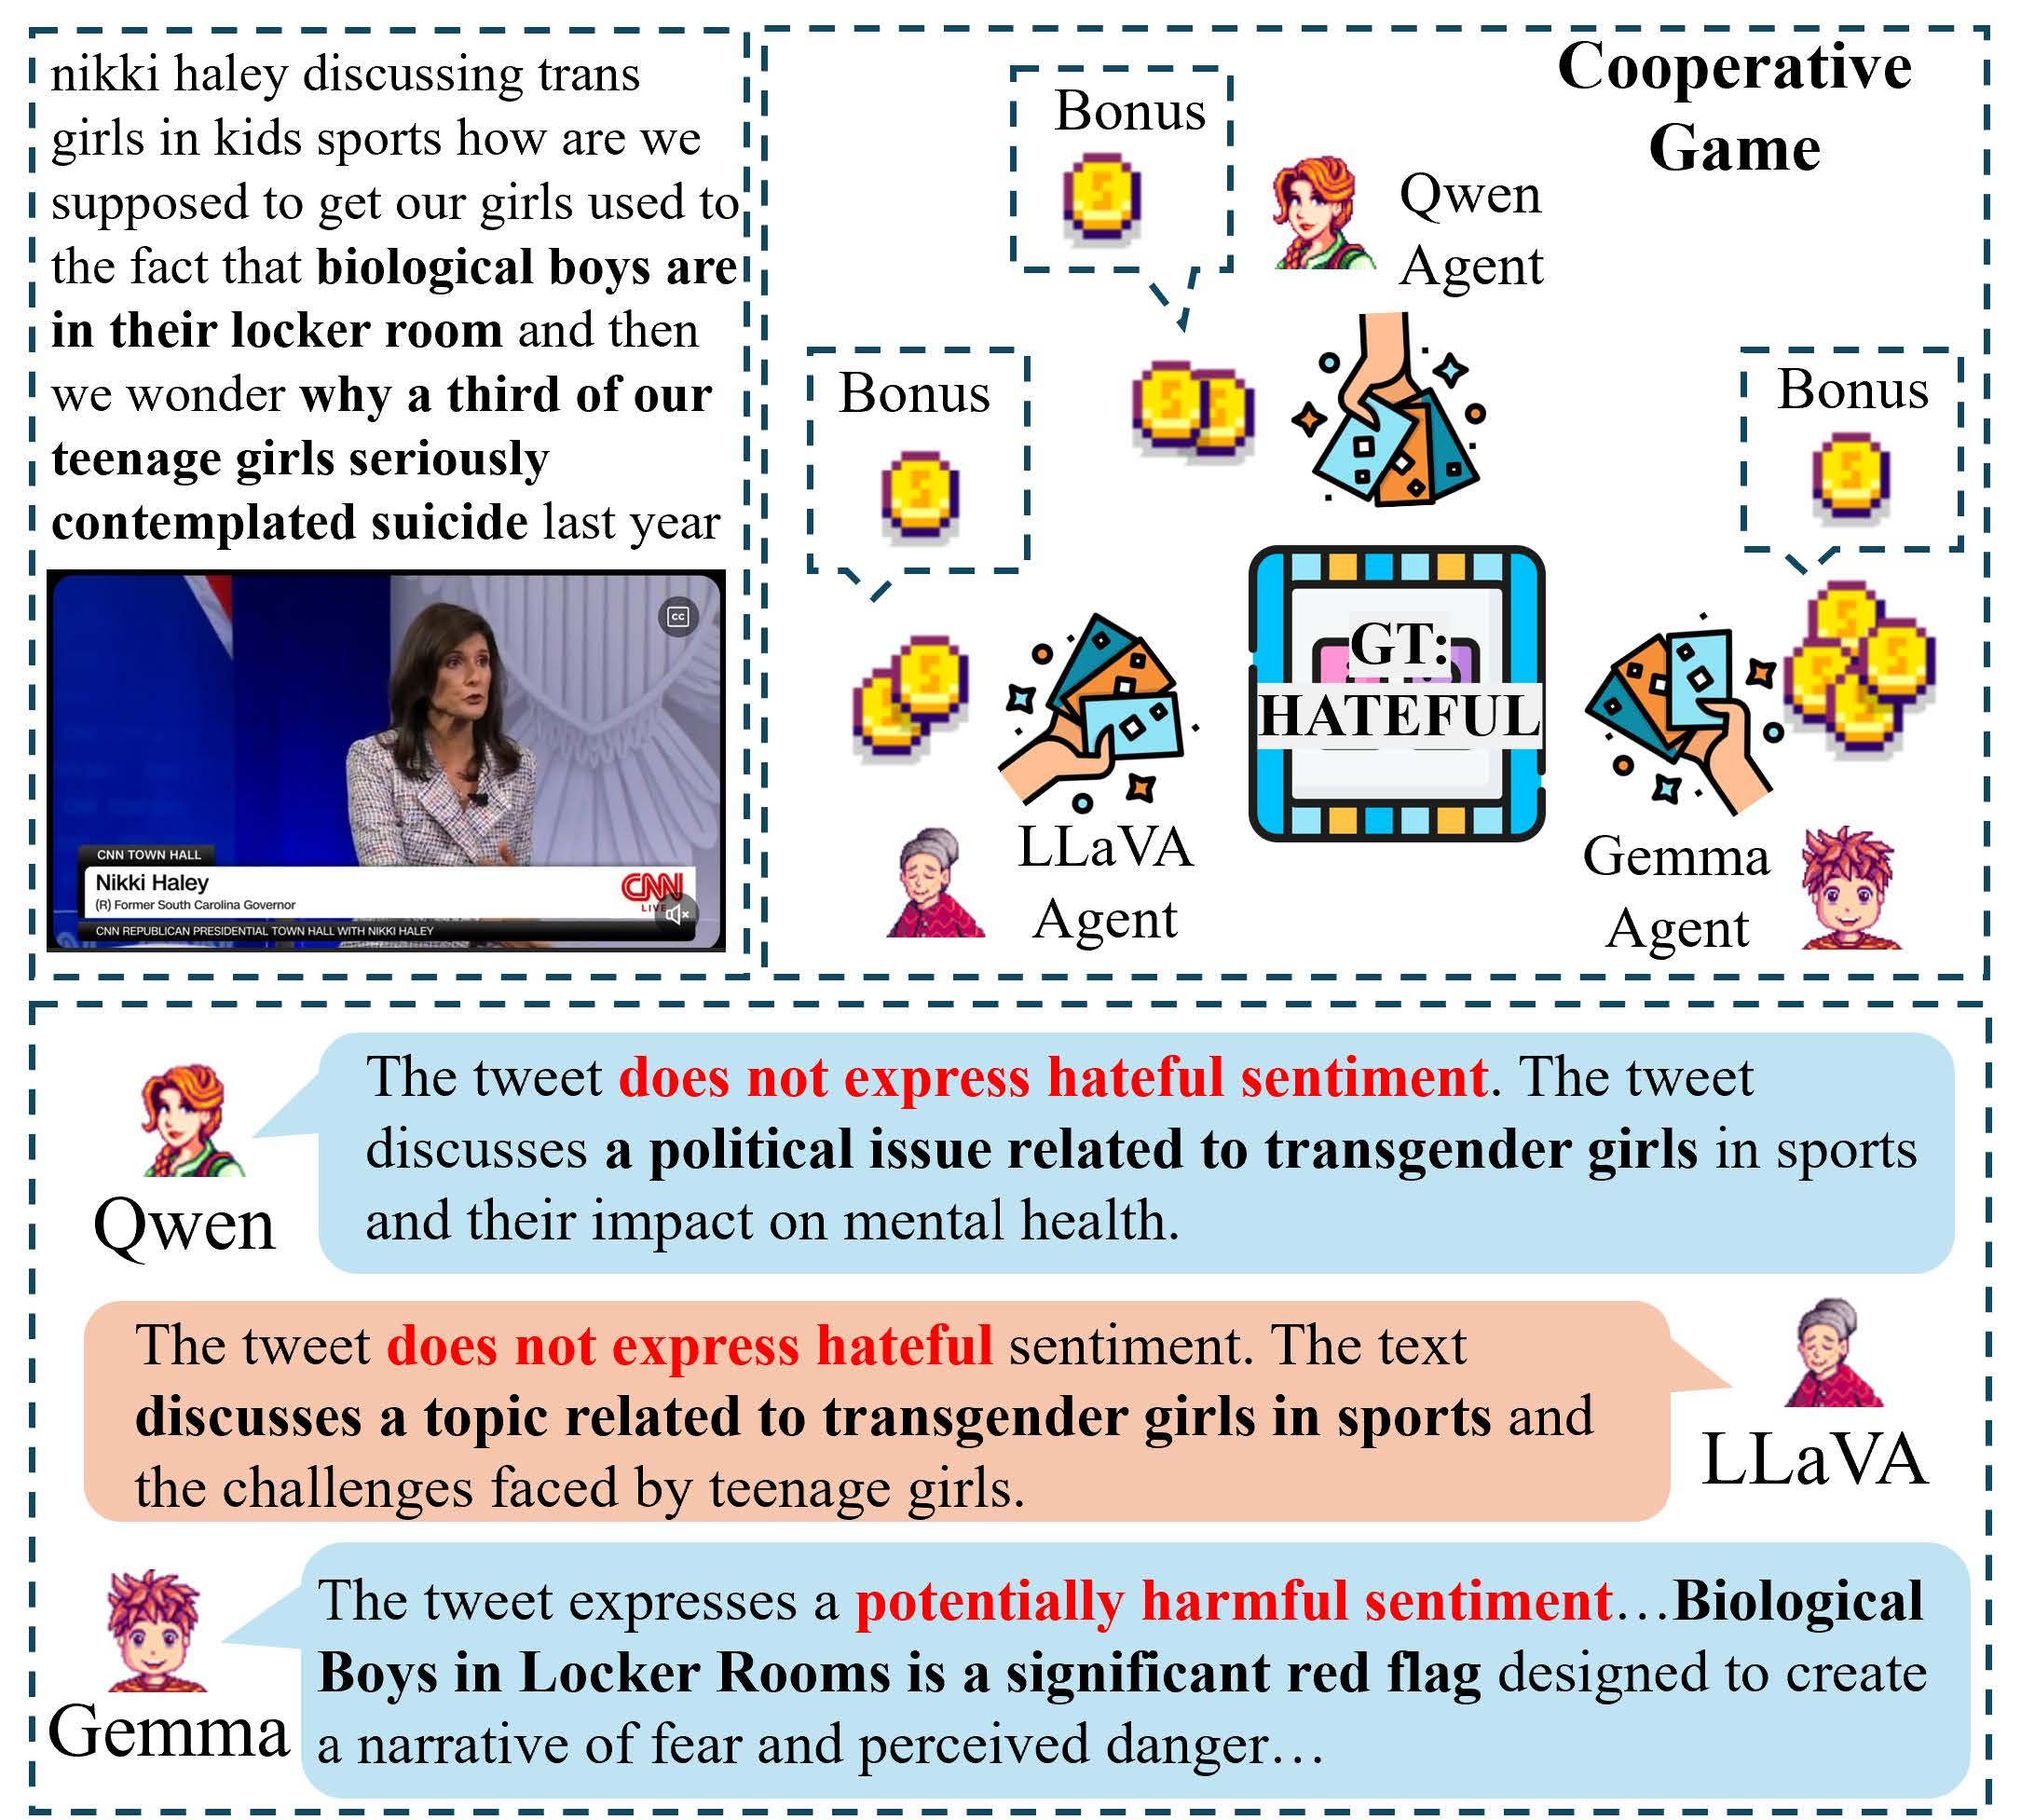
\includegraphics[width=0.8\linewidth]{fig_1.jpeg}
    \caption{\textbf{Illustration of model bias in Hateful Meme Classification}. For the hateful meme about Nikki Haley, three LMMs (Qwen, Gemma,
    LLaVA) present varied interpretations; only Gemma identifies the correct label,
    guiding the cooperative framework toward the accurate answer.}
    \label{fig:bias}
\end{figure}

Both of these ensemble strategies are flawed. Voting fails when
several models happen to share the same underlying bias, since the majority can be
confidently wrong together. Debate-based systems shift the burden onto the judge model,
which itself may be biased, so a bad judge can steer the whole debate toward the wrong
answer. The authors illustrate this with a real example, shown in Figure~\ref{fig:bias},
involving a meme about Nikki Haley discussing transgender girls in sports: two of the
three LMMs tested (Qwen and LLaVA) misread the meme as neutral, while only Gemma
correctly detected the underlying hostility. In this situation, majority voting would
have picked the wrong label, and a debate judge influenced by the majority opinion could
easily be misled as well.

To get around this, we turn to game theory, specifically the concept of a
\textbf{Nash equilibrium}, where every participant in a system reaches a stable strategy that
none of them wants to unilaterally deviate from. Applying this idea directly to model
ensembling is not straightforward, though, because simply letting each model optimize
its own prediction does not automatically produce agreement across models. The paper's
proposed system, GECO (Game-theoretic multi-agEnt Collaboration framewOrk), tries to
solve this by treating the combination of LMMs as a cooperative game: each model is an
``agent,'' and a reward structure is designed so that agents are incentivized not just
for being individually correct, but for reaching agreement with each other on the correct
label. On top of this, the authors add an efficient training procedure and a stabilizing
penalty term so the whole system converges reliably instead of oscillating.

The contributions of the paper can be summarized as follows:
\begin{itemize}
    \item It is, as far as the authors state, the first work to frame multi-agent
    collaboration for hateful meme detection using game-theoretic principles.
    \item It proposes GECO, which combines multiple LMMs and pushes them toward mutual
    agreement on the correct label through a designed reward (``bonus'') scheme, along
    with an efficient and stable training method.
    \item It shows through experiments on multiple public benchmarks that GECO
    outperforms existing state-of-the-art detection methods.
\end{itemize}
\section{Background and Related Work}

\subsection{Hateful Meme Classification}

Detecting hateful memes is a challenging task because the harmful meaning often emerges
only from the combination of image and text, rather than from either one alone. Several
benchmark datasets have been released over the years to push progress in this area, and
these releases have also made clear how difficult the task really is. Early detection
systems used dual-stream architectures, encoding the image and text separately and then
combining (``fusing'') the two streams late in the pipeline, or they fine-tuned existing
multimodal backbones for the task. However, these attention-based and shallow-fusion
approaches often struggle with cues that depend on implicit or culture-specific context,
which is very common in hateful content.

More recent work shifts toward using LMMs to generate explanations or rationales that
can either be distilled into smaller models or used directly to support a final decision.
A key limitation the authors point out is that LMMs carry their own inherent biases, and
these biases can create contradictions when multiple models are used together to detect
hate speech. When a majority of the models in a system share the same bias, simple
strategies such as majority voting stop being effective, since the majority opinion is
confidently wrong.

\subsection{Game Theory}

Game theory is a mathematical framework for finding optimal decisions when multiple
``players'' interact, each with their own goals. The central solution concept used in
game theory is the \textbf{Nash equilibrium}, a stable state in which no player can improve
their own outcome by changing their strategy alone, assuming all other players keep their
strategies fixed.

Game-theoretic formulations are generally split into two branches. Cooperative game
theory focuses on how a group of players should split a predetermined shared value among
themselves, and it provides standard tools for handling binding agreements between
players. Non-cooperative game theory, on the other hand, is used to model competitive,
strategic scenarios, and it has been applied successfully to games such as poker,
StarCraft, Go, and Diplomacy, where independent agents compete or negotiate under fixed
rules.

When multiple models are combined for a classification task, this combination can also be
viewed as a kind of non-cooperative game between the models. However, the authors note
that simply applying standard game-theoretic tools in this setting does not guarantee
that the models will reach agreement -- it can still result in unstable decisions and
biases that persist across the group. This gap is exactly what motivates the design of
GECO: a framework that combines specialized agents with an objective that explicitly
rewards consensus, aiming for bias-aware collaborative decisions across multiple LMMs.

\section{Method}

Our reproduction of the proposed approach, GECO, is organized as follows. We first
describe how all agents in the framework are defined and what actions they take to
participate in the collaborative game. We then explain the optimization strategy used to
reduce bias across the different models and to steer them toward consistent, agreed-upon
predictions. Figure~\ref{fig:overview} gives an overview of the overall architecture,
showing how the reasoning agents, the learnable agent, and the master agent interact
within a regularized game, coordinated through a mixed bonus scheme and an efficient
policy-learning procedure.

\begin{figure}[h]
    \centering
    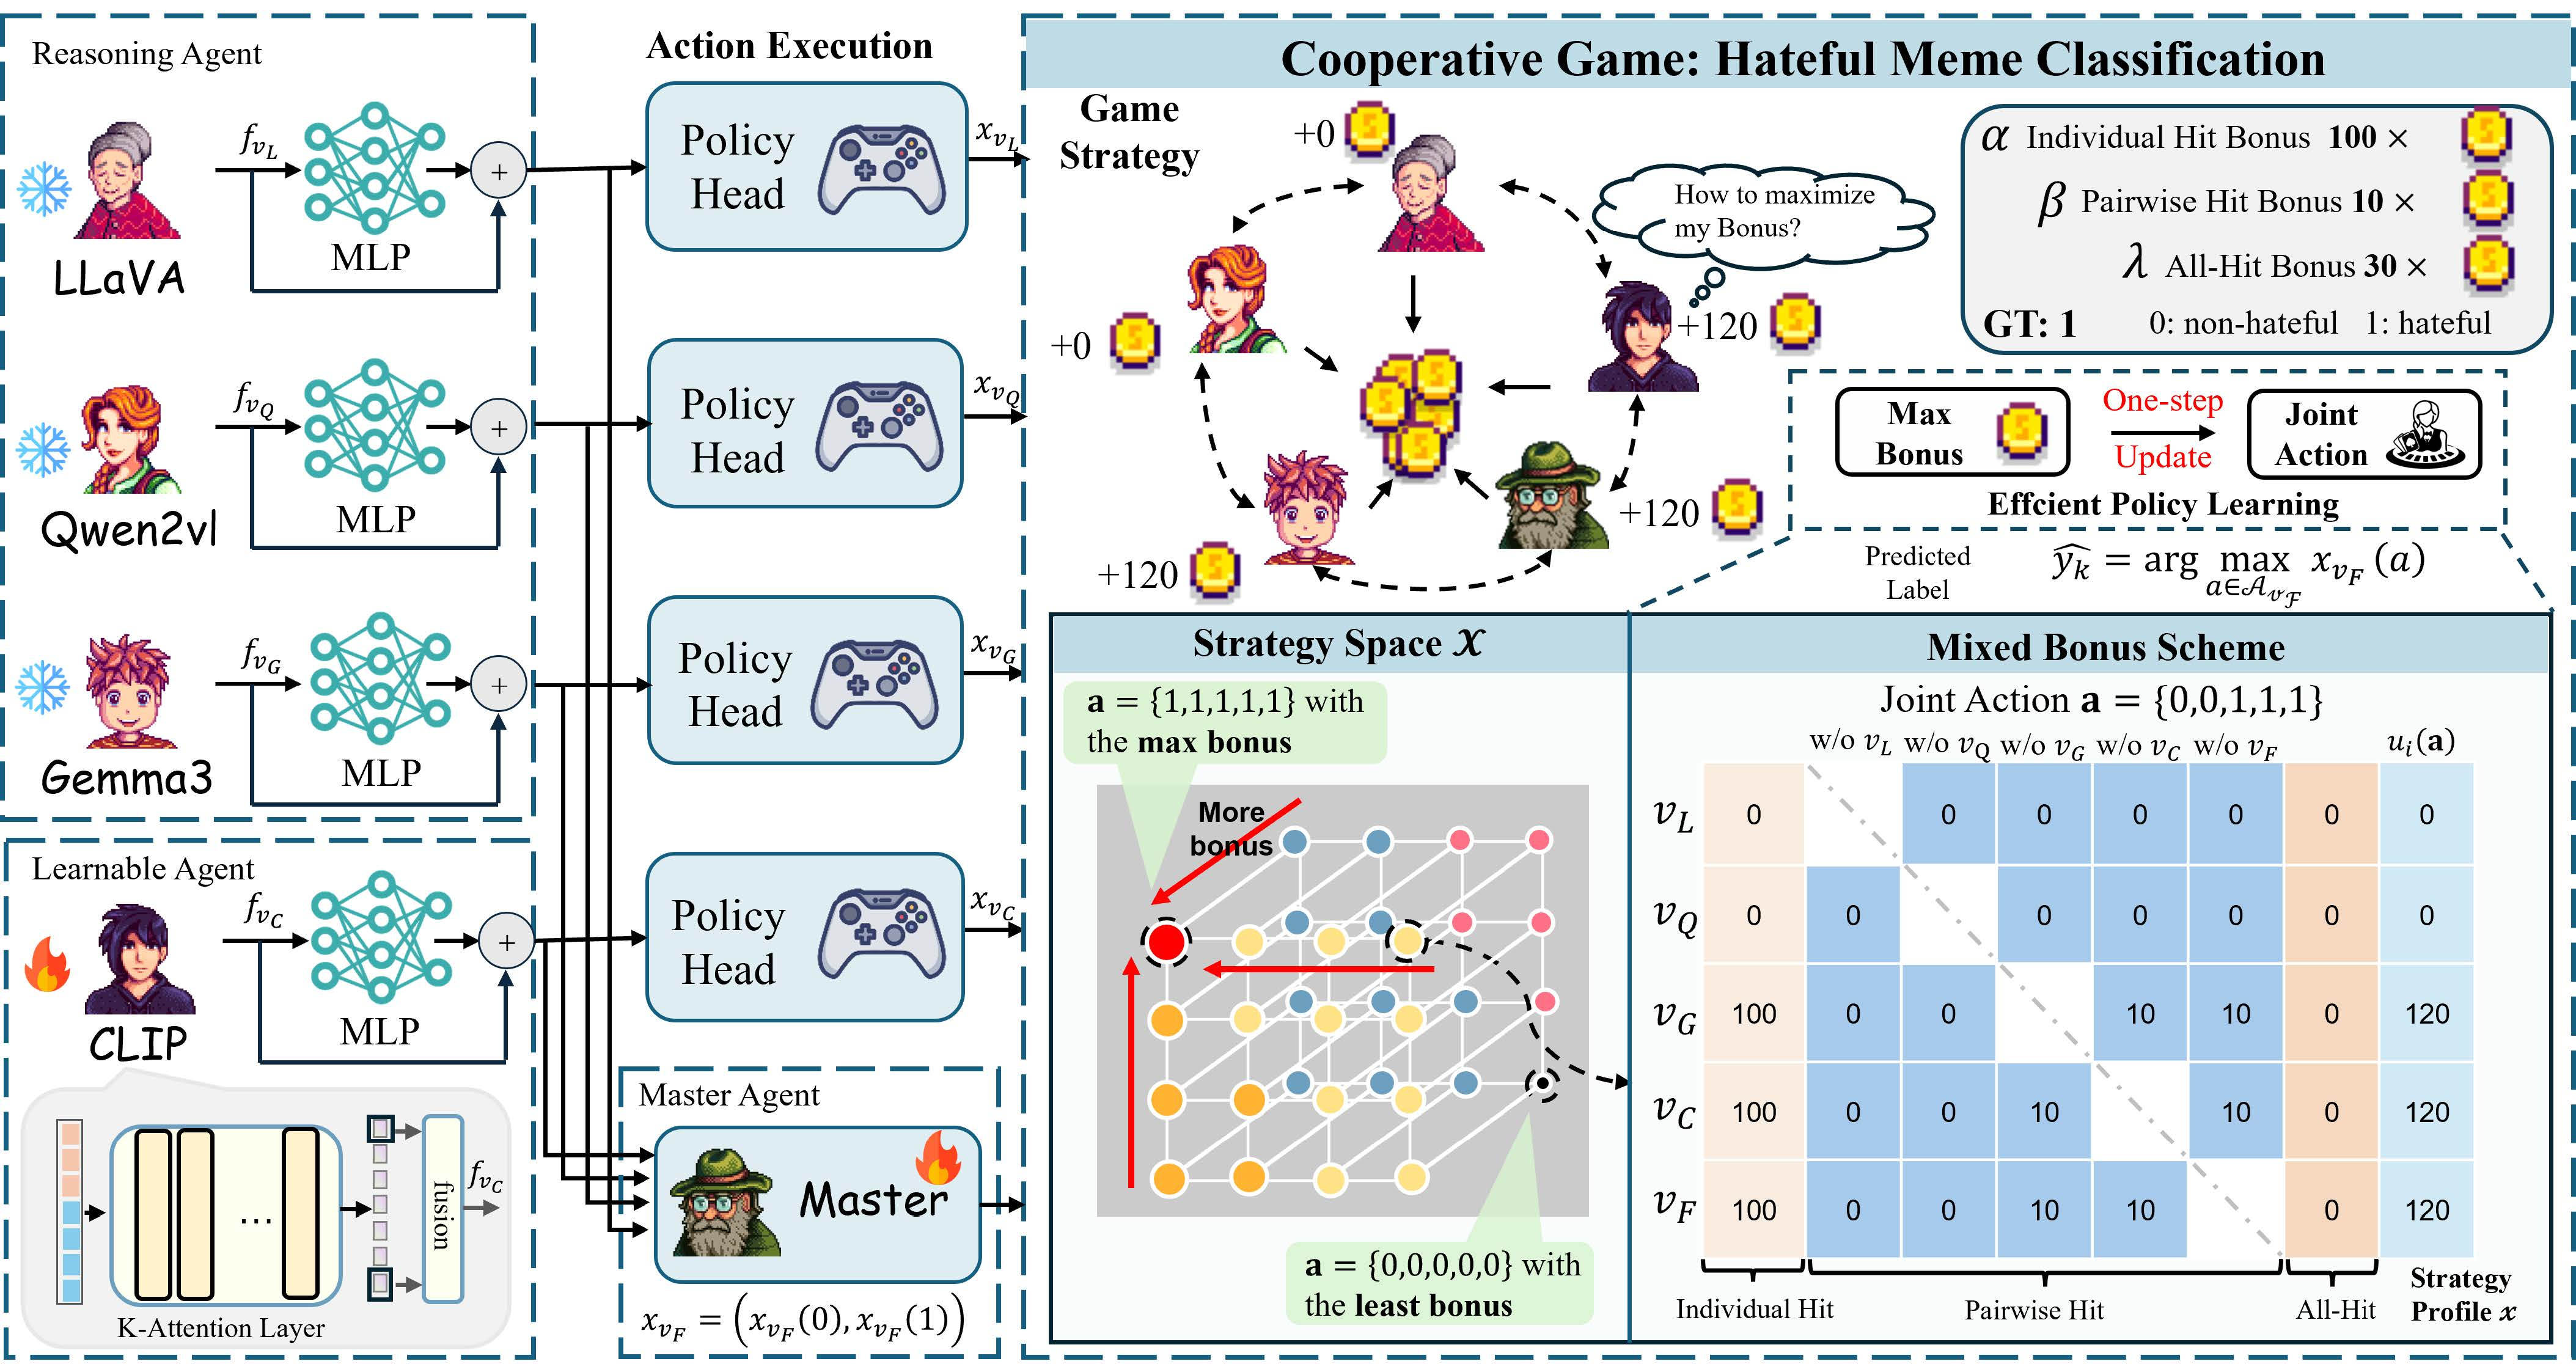
\includegraphics[width=\linewidth]{fig_2.jpeg}
    \caption{Overview of the GECO framework, reproduced from the original paper.
    Reasoning agents (LLaVA, Qwen2-VL, Gemma3) and a learnable CLIP-based agent interact
    under a regularized normal-form game, coordinated by a master agent.}
    \label{fig:overview}
\end{figure}

\subsection{Game Agents Definition}

\subsubsection{\textbf{Agents Introduction. \newline }}

The GECO framework defines three types of agents that participate in the game: the
\textit{reasoning agent}, \textit{the learnable agent}, and the \textit{master agent}.

\textbf{Reasoning agents.} To capture complementary ways of interpreting a meme, the
authors select three widely-used LMMs as reasoning agents: Qwen2-VL ($v_Q$), LLaVA-1.5
($v_L$), and Gemma3 ($v_G$). Each of these models brings its own strengths in multimodal
understanding, and using three different backbones together is meant to reduce the risk
that a single model's blind spot dominates the final decision.

Before the actual game starts, all three reasoning agents are first adapted to the task
using lightweight LoRA fine-tuning ~\cite{hu2022lora}. Once the game begins, however, these agents are kept
frozen -- their weights no longer update. This preserves the reasoning ability each model
already has and ensures they act as a stable source of features for the rest of the
system. For a labeled training sample $\xi_k$, each LMM is trained to output a single
token that represents the label $s(y_k)$ in text form, using a standard language modeling
loss:

\begin{equation}
\mathcal{L}_i^{\text{LMM}} = -\sum_{k=1}^{N} \log p_{\theta_i}\big(\hat{y}_k^{\text{LMM}} = s(y_k) \mid \xi_k\big),
\end{equation}

where $p_{\theta_i}$ is the token-level probability distribution produced by the LMM with
its LoRA adapters. Each reasoning agent $i \in \{v_Q, v_L, v_G\}$ produces a hidden
representation $f_i^k = h_i(\xi_k)$, where $h_i(\cdot)$ denotes that model's backbone, and
this representation corresponds to the hidden state of the last token generated. This
hidden representation is then projected into a shared decision space $\mathcal{D}$ to
produce the agent's final representation:

\begin{equation}
z_i^k = \phi_i(f_i^k) \in \mathbb{R}^D.
\end{equation}

\textbf{Learnable agent.} Since the three reasoning agents are frozen once the game
begins, the authors add a fourth, learnable agent $v_C$, whose purpose is to keep
adapting its understanding of strategy throughout training. For this role, they choose a
CLIP-based model, mainly because it has relatively few parameters while still offering
strong multimodal representation ability, keeping computational cost manageable.

Given a labeled sample $\xi_k$, the CLIP text encoder converts the text $T_k$ into token
embeddings $S_k = \{s_1, \dots, s_n, s_{\text{cls}}\}$, while the CLIP image encoder
converts the image $I_k$ into patch embeddings $V_k = \{v_{\text{cls}}, v_1, \dots,
v_m\}$. These two sequences are concatenated and passed through a $K$-layer Transformer
encoder to model interactions between the image and text modalities. The resulting
aggregate vectors, $\tilde{v}_{\text{cls}}$ and $\tilde{s}_{\text{cls}}$, are then combined
using a lightweight fusion step:

\begin{equation}
(p_s, p_v) = \text{softmax}\big(W_f([\tilde{s}_{\text{cls}}; \tilde{v}_{\text{cls}}])\big), \quad
f_{v_C}^k = p_s\, \tilde{s}_{\text{cls}} + p_v\, \tilde{v}_{\text{cls}},
\end{equation}

where $W_f$ is a learnable weight matrix. This fused feature is then projected into the
same shared decision space:

\begin{equation}
z_{v_C}^k = \phi_{v_C}(f_{v_C}^k) \in \mathbb{R}^D.
\end{equation}

\textbf{Master agent.} The final agent, the [master agent] $v_F$, is responsible for
combining the representations from all other agents and producing the system's final
prediction. It acts as the ultimate decision-maker in the game, and importantly, its own
payoff depends not just on its own action but also on the actions taken by the other
agents -- this dependency is what makes the overall decision more robust to any single
agent's bias. The projected features from all other agents are simply concatenated to
form the master agent's representation:

\begin{equation}
z_{v_F}^k = [\, z_{v_L}^k;\, z_{v_Q}^k;\, z_{v_C}^k;\, z_{v_G}^k \,] \in \mathbb{R}^{4D}.
\end{equation}

\subsubsection{\textbf{Action Execution.} \newline}

Each agent $v_i \in \mathcal{V} = \{v_L, v_Q, v_C, v_G, v_F\}$ maintains its own policy
$\pi_i$ over a binary action space $\mathcal{A}_i = \{0, 1\}$, where an action of $0$
means ``non-hateful'' and $1$ means ``hateful.'' Together, the actions chosen by all five
agents form a joint action set $\mathcal{A}^5 = \{a_{v_L}, a_{v_Q}, a_{v_C}, a_{v_G},
a_{v_F}\}$. Each agent's policy is a probability distribution over its two possible
actions, conditioned on the input sample: $\pi_i(\cdot \mid \xi_k) \in \Delta(\mathcal{A}_i)$.

To turn an agent's internal representation $z_i^k$ into an actual action preference, the
authors pass it through an agent-specific policy head $\psi_i$ to obtain logits, and then
apply a temperature-scaled softmax:

\begin{equation}
\ell_i^k = \psi_i(z_i^k) \in \mathbb{R}^{|\mathcal{A}_i|}, \qquad
\pi_i(a_i \mid \xi_k) = \frac{\exp\big((\ell_i^k)_{a_i}/\tau_i\big)}{\sum_{a' \in \mathcal{A}_i} \exp\big((\ell_i^k)_{a'}/\tau_i\big)}.
\end{equation}

The temperature parameter $\tau_i$ controls how ``confident'' or ``spread out'' each
agent's action distribution is. Using this policy, the authors define what they call the
[mixed bonus vector] $x_i$ of agent $v_i$, which is simply the probability the agent
assigns to each possible action:

\begin{equation}
x_i = \big(x_i(a_1), x_i(a_2), \dots, x_i(a_{|\mathcal{A}_i|})\big) \in \mathcal{X}_i,
\end{equation}

where $\mathcal{X}_i$ represents the space of possible strategies for agent $i$. Taking
the full collection of all agents' strategies together, $x = \{x_i \mid i \in
\mathcal{V}\}$, is referred to as the strategy profile of the whole system. The final
predicted label $\hat{y}_k$ for a given sample is simply whichever action the master agent
assigns the highest probability to:

\begin{equation}
\hat{y}_k = \arg\max_{a \in \mathcal{A}_{v_F}} x_{v_F}(a).
\end{equation}

In other words, while every agent maintains and updates its own strategy throughout
training, it is ultimately the master agent's policy that determines the system's output
prediction -- the other agents influence this outcome indirectly, through the shared
optimization process described in the next subsection.

\subsection{Game Strategy}

\subsubsection{\textbf{Mixed Bonus Scheme.} \newline}

Most applications of game theory focus on optimizing each player's individual
performance. The authors take a different angle here: since the goal is to overcome
biases that are shared across models, GECO's reward design instead prioritizes
[overall consensus] among the agents, encouraging both individual correctness and
mutual agreement on the correct label at the same time.

Given a joint action $a = \{a_{v_L}, a_{v_Q}, a_{v_C}, a_{v_G}, a_{v_F}\} \in
\mathcal{A}^5$ and the true label $y_k$ for a sample, the mixed bonus (reward) received
by agent $i$ is defined as:

\begin{equation}
u_i(a_i, a_{-i}) = \alpha \cdot \mathbb{I}(a_i = y_k)
+ \lambda \sum_{j \in \mathcal{V}\setminus\{i\}} \mathbb{I}(a_i = y_k)\,\mathbb{I}(a_j = y_k)
+ \beta \cdot \mathbb{I}\big(\forall j \in \mathcal{V},\, a_j = y_k\big),
\end{equation}

where $\mathbb{I}(\cdot)$ is the indicator function (equal to 1 if the condition is true,
0 otherwise), and $a_{-i}$ represents the actions chosen by all agents other than $i$.
This reward has three distinct components:

\begin{itemize}
    \item An individual hit bonus $\alpha$, rewarding an agent simply for predicting the
    correct label on its own, regardless of what other agents do.
    \item A pairwise hit bonus $\lambda$, which rewards an agent extra for every other
    agent that \emph{also} happens to predict the correct label at the same time --
    encouraging agreement between pairs of agents.
    \item An all-hit bonus $\beta$, which is only awarded when \emph{every single agent}
    in the system predicts the correct label simultaneously, rewarding full consensus.
\end{itemize}

The overall goal during training is to maximize the expected value of this reward for
every agent. Given the strategy profile $x = \{x_j\}_{j \in \mathcal{V}}$, the expected
utility of agent $i$ is computed by summing the reward over every possible combination of
actions across all agents, weighted by how likely that combination is under the current
strategies:

\begin{equation}
U_i(x_i, x_{-i}) = \sum_{a \in \times_{j \in \mathcal{V}} \mathcal{A}_j} u_i(a) \cdot \prod_{j \in \mathcal{V}} x_j(a_j),
\end{equation}

where $a$ denotes one particular joint action drawn from the full joint action space. In
short, this reward structure is designed so that an agent cannot maximize its own expected
payoff by acting alone -- its best outcome depends on other agents also converging toward
the correct label, which is precisely the mechanism meant to push the whole system toward
a shared, correct consensus rather than isolated individual guesses.

\subsubsection{\textbf{Efficient Policy Learning.} \newline}

The aim during training is for every agent to converge on the overall best strategy
through repeated sampling of actions. However, the authors point out that the standard
way of doing this in game theory is not ideal here, mainly because each agent only has a
binary choice (hateful or non-hateful), and any incorrect classification simply
contributes nothing useful to the overall expected reward. Given this, the authors
restrict sampling so that only the [correct action] is considered for each agent, rather
than sampling across the full action space.

This restriction brings two practical benefits. First, it reduces computation, since the
system no longer needs to evaluate outcomes for incorrect actions that would not
contribute meaningfully anyway. Second, because the effective action space is smaller,
the authors are able to use single-step updates instead of repeated multi-sample
updates, which also avoids extra noise that multiple sampling rounds would normally
introduce.

To formalize this, the authors define the [expected conditional utility] $U_i(a_i,
x_{-i})$, representing the expected reward agent $i$ would receive for taking a specific
action $a_i$, assuming all other agents continue to act according to their current
strategies $x_{-i}$:

\begin{equation}
U_i(a_i, x_{-i}) = \sum_{a_{-i} \in \times_{j \in \mathcal{V}\setminus\{i\}} \mathcal{A}_j} u_i(a_i, a_{-i}) \cdot \prod_{j \in \mathcal{V}\setminus\{i\}} x_j(a_j).
\end{equation}

In practice, this computation is implemented efficiently using vectorized tensor
operations, producing the expected reward for each possible action all at once, rather
than looping over them individually.

To help training actually converge toward a [Nash equilibrium] rather than oscillating
indefinitely, the authors add a regularization term based on prior theoretical work. This
gives a regularized advantage vector $F_i^x$, along with its individual scalar components
$F_i^x(a_i)$:

\begin{equation}
F_i^x = -\nabla_{x_i} u_i(x) + \eta \log(x_i), \qquad
F_i^x(a_i) = -U_i(a_i, x_{-i}) + \eta \log x_i(a_i),
\end{equation}

where $\eta$ is a balance parameter controlling how strongly this regularization affects
the update. To make training more stable, the regularized advantage is then centered by
subtracting a baseline value $B_i$, computed under a simple baseline strategy $\hat{x}_i$
(for example, a uniform distribution over actions):

\begin{equation}
B_i = \langle F_i^x, \hat{x}_i \rangle = \sum_{a_i} \hat{x}_i(a_i) F_i^x(a_i).
\end{equation}

This gives the final centered advantage vector:

\begin{equation}
A_i = F_i^x - B_i \mathbf{1},
\end{equation}

where $\mathbf{1}$ denotes a vector of all ones. Finally, the [Regularized Nash Advantage
loss] $\mathcal{L}_{\text{RNA}}(x)$ used to train agent $i$ is defined as the inner
product between the agent's current strategy $x_i$ and a stop-gradient version of its
centered advantage vector:

\begin{equation}
\mathcal{L}_{\text{RNA}}(x) = \sum_{i \in \mathcal{V}} \big\langle \text{sg}(F_i^x - \langle F_i^x, \hat{x}_i \rangle \mathbf{1}),\ x_i \big\rangle
= \sum_{i \in \mathcal{V}} \langle \text{sg}\, A_i,\ x_i \rangle.
\end{equation}

The stop-gradient operator $\text{sg}(\cdot)$ simply treats $A_i$ as a fixed constant
during backpropagation, which simplifies the gradient computation and improves numerical
stability. Minimizing this loss pushes each agent's strategy toward actions that have a
positive advantage, gradually steering the whole system toward maximizing overall
benefit.

\subsubsection{\textbf{Regularization and Final Objective.} \newline}

Even with the regularized advantage formulation above, updates during training can still
oscillate from step to step. To reduce this instability, the authors introduce an
additional regularization step that keeps the current policy close to a slowly-changing
reference version of itself.

Specifically, let $p = \pi_{v_F}$ denote the master agent's current policy. The authors
maintain a separate reference policy $q$, updated using an [exponential moving average
(EMA)] of the current policy over time:

\begin{equation}
q_t \leftarrow \mu\, q_{t-1} + (1 - \mu)\, p_t,
\end{equation}

where $\mu$ controls how slowly the reference policy $q$ is allowed to change -- a value
closer to 1 makes $q$ update more slowly and act as a more stable anchor. To keep the
current policy $p$ from drifting too far from this slowly-moving reference, the authors
define a symmetric KL-style regularization term:

\begin{equation}
J_\gamma(p, q) = (1 - \gamma)\, D_{\text{KL}}(q \parallel p) + \gamma\, D_{\text{KL}}(p \parallel q),
\end{equation}

where $D_{\text{KL}}(\cdot \parallel \cdot)$ is the standard Kullback-Leibler divergence,
and $\gamma$ is a mixing coefficient that balances the two directions of the divergence.
Using both terms symmetrically (rather than just one direction) helps prevent the policy
from either changing too abruptly or getting stuck too rigidly close to the reference.

Combining this stabilizing term with the Regularized Nash Advantage loss from the
previous subsection gives the final training objective used to optimize the entire GECO
framework:

\begin{equation}
\mathcal{L} = \mathcal{L}_{\text{RNA}} + J_\gamma(p, q),
\end{equation}

where $\mathcal{L}_{\text{RNA}}$ is responsible for pushing the agents toward the
game-theoretic consensus objective described earlier, while $J_\gamma$ acts purely as a
smoothing term, ensuring that the master agent's policy evolves gradually rather than
jumping erratically between updates during training.

\section{Experimental Setup}

The experiments in the paper are conducted on five publicly available datasets: Hateful
Meme, PrideMM, MultiOff, HarMeme, and MAMI. These datasets cover a range of meme styles
and target different forms of harmful content, which allows the authors to test how well
GECO generalizes across different data conditions, including low-resource settings such
as MultiOff, which contains fewer than 500 samples.

\subsection{Baselines}

The authors compare GECO against two broad categories of existing methods:

\begin{itemize}
    \item \textbf{CLIP-based methods}: these rely on the CLIP model as a shared
    vision-language backbone, and include CLIP~\cite{radford2021clip} itself,
    MOMENTA~\cite{pramanick2021momenta}, Hate-CLIPper~\cite{kumar2022hateclipper},
    MemeCLIP~\cite{shah2024memeclip}, and RGCL~\cite{mei2024rgcl}.
    \item \textbf{LMM-based methods}: these use large multimodal models for reasoning
    about meme content, and include IntMeme~\cite{hee2025intmeme},
    ExplainHM~\cite{lin2024explainhm}, Mod-Hate~\cite{cao2024modhate},
    LoReHM~\cite{huang2024lorehm}, M2KE~\cite{lu2025m2ke}, and
    RA-HMD~\cite{mei2025rahmd} -- the last of which was the previous state-of-the-art
    model before GECO.
\end{itemize}

\subsection{Implementation Details}

For the reasoning agents, the authors use three LMMs of different sizes: LLaVA-1.5-13B~\cite{liu2023llava},
Qwen2-VL-7B~\cite{wang2024qwen2vl}, and Gemma3-4B~\cite{gemma2025gemma3}, deliberately spanning from 4B to 13B parameters. This is a
departure from prior work, which typically relies only on larger 7B--13B backbones --
here, including a smaller model as well lets the authors test how well the cooperative
framework scales across different model sizes and computational budgets.

All agent representations are projected into a shared decision space of dimensionality
$D = 768$. Training uses the AdamW optimizer, with a learning rate of $2 \times 10^{-5}$
for all non-CLIP parameters and a higher rate of $5 \times 10^{-5}$ for the CLIP-related
components. For the regularized advantage term described in the Method section, the
balance parameter is set to $\eta = 0.35$. The three bonus terms in the mixed bonus
scheme are set to $\alpha = 1.0$ (individual hit), $\lambda = 0.5$ (pairwise hit), and
$\beta = 1.0$ (all-hit), while the mixing coefficient for the KL regularization term is
set to $\gamma = 0.5$.

Following the evaluation protocol used in prior work, the authors report three standard
metrics: Accuracy (Acc), F1-Score (F1), and Area Under the Curve (AUC).

\section{Results and Discussion}

\subsection{Main Results}

Table~\ref{tab:main-results} summarizes how GECO compares against both CLIP-based and
LMM-based baseline methods across all five benchmark datasets. A few key observations
stand out from these results.

First, GECO achieves the best performance on every single benchmark, which supports the
authors' central claim that treating multi-agent collaboration as a cooperative game
genuinely helps reduce inconsistencies between heterogeneous agents. The improvement is
especially large on PrideMM, where GECO surpasses the previous best method, RA-HMD, by
roughly 4.7 percentage points in accuracy. On MAMI, GECO reaches about 81.5\% accuracy
and 82.8\% F1, again ahead of all prior methods. The gains are even more pronounced on
MultiOff, a dataset with fewer than 500 samples that is historically difficult for
single-model systems -- GECO exceeds RA-HMD by more than 7 percentage points in accuracy
here, suggesting that the cooperative framework is particularly useful in low-resource
settings, where models can compensate for each other's blind spots by sharing
complementary visual and textual cues.

Second, LMM-based methods generally outperform older CLIP-based methods, which lines up
with expectations given the stronger reasoning ability of LMMs on subtle, implicit
content. However, the authors point out that relying on a single LMM's perspective tends
to lock in that model's own biases, which can hurt both fairness and robustness. GECO's
advantage over LMM-based baselines suggests that this bias is not an unavoidable
limitation -- it can be substantially reduced by deliberately introducing heterogeneity
(different backbones) together with a collaborative mechanism.

Third, GECO also outperforms existing debate-based ensemble methods such as ExplainHM and
M2KE. While these methods do introduce some interaction between agents, they rely on
fixed dialogue rules or on a separate judge model, both of which can limit stability or
introduce their own bias. GECO's game-theoretic formulation instead allows agents to
adapt to each other more flexibly, which the results suggest leads to stronger and more
reliable consensus.

\begin{table*}[t]
\centering
\caption{Comparison with baseline systems across five benchmark datasets (reproduced from
the original paper). Best performance in each column is shown in bold.}
\label{tab:main-results}
\begin{tabular}{ll|cc|cc|cc|cc|cc}
\toprule
\textbf{Category} & \textbf{Method} & \multicolumn{2}{c|}{\textbf{PrideMM}} & \multicolumn{2}{c|}{\textbf{HatefulMemes}} & \multicolumn{2}{c|}{\textbf{MAMI}} & \multicolumn{2}{c|}{\textbf{HarMeme}} & \multicolumn{2}{c}{\textbf{MultiOff}} \\
 & & Acc & F1 & Acc & AUC & Acc & AUC & Acc & AUC & Acc & F1 \\
\midrule
\multirow{5}{*}{CLIP-Based}
 & CLIP (2021)         & 72.39 & 72.33 & 72.04 & 79.81 & 77.70 & 68.40 & 76.78 & 82.63 & 62.41 & 48.14 \\
 & MOMENTA (2021)      & 72.23 & 71.78 & 61.34 & 69.17 & 72.10 & 81.68 & 80.48 & 86.32 & --    & --    \\
 & Hate-CLIPper (2022) & 75.53 & 74.08 & 76.10 & 85.48 & 74.80 & 87.20 & 84.80 & 89.72 & 62.40 & 54.80 \\
 & MemeCLIP (2024)     & 76.06 & 76.09 & --    & --    & --    & --    & 84.72 & 83.74 & --    & --    \\
 & RGCL (2024)         & 76.34 & 76.50 & 78.92 & 87.04 & 78.40 & 89.40 & 87.03 & 91.91 & 67.13 & 58.11 \\
\midrule
\multirow{6}{*}{LMM-Based}
 & ExplainHM$^\dagger$ (2024) & --    & --    & 75.60 & --    & --    & --    & 87.00 & --    & --    & --    \\
 & Mod-Hate (2024)     & --    & --    & 59.07 & 64.69 & 61.10 & 67.20 & 69.85 & 73.26 & --    & --    \\
 & LoReHM (2024)       & --    & --    & 65.60 & --    & 75.40 & --    & 73.73 & --    & --    & --    \\
 & M2KE$^\dagger$ (2025) & --  & --    & 75.76 & 75.62 & 75.85 & --    & --    & --    & --    & --    \\
 & IntMeme (2025)      & --    & --    & 71.52 & 81.50 & 72.30 & 81.89 & 81.92 & 89.35 & --    & --    \\
 & RA-HMD (2025)       & 78.10 & 78.70 & 82.10 & 91.10 & 79.90 & 90.40 & 88.10 & 93.20 & 71.11 & 64.80 \\
\midrule
 & \textbf{GECO}       & \textbf{82.84} & \textbf{82.84} & \textbf{84.35} & \textbf{91.57} & \textbf{81.50} & \textbf{91.80} & \textbf{89.11} & \textbf{93.95} & \textbf{78.52} & \textbf{77.90} \\
\bottomrule
\end{tabular}
\end{table*}

\subsection{Ablation Study}

To understand how much each part of GECO's architecture actually contributes, the authors
run a series of ablation experiments, summarized in Table~\ref{tab:ablation}, on the
PrideMM and MultiOff datasets.

In the single-agent ablations, removing the master agent $v_F$ causes by far the largest
drop in performance, which confirms that treating the classifier itself as an active
player in the cooperative game -- rather than just a passive aggregator -- is essential to
the framework's design. Removing the core reasoning agent $v_L$ (LLaVA) causes the second
largest drop, reflecting its strong role in vision-language understanding generally. The
learnable agent $v_C$ (CLIP) also matters, primarily because it contributes cross-modal
alignment that the other agents do not directly provide, while the two remaining
reasoning agents, $v_Q$ (Qwen) and $v_G$ (Gemma), contribute additional contextual and
linguistic diversity.

Beyond these individual effects, the two-agent ablations reveal something more
interesting: removing any \emph{pair} of agents together causes a drop in performance that
is noticeably larger than simply adding up the two individual removal effects. This
suggests that the agents are not just contributing independently -- they depend on each
other in a genuinely synergistic way, which supports the authors' argument that the
reward design specifically encourages cooperative interaction rather than agents just
working in isolation.

\begin{table}[h]
\centering
\caption{Ablation study on PrideMM and MultiOff datasets (reproduced from the original
paper).}
\label{tab:ablation}
\begin{tabular}{ll|cc|cc}
\toprule
\textbf{Category} & \textbf{Mode} & \multicolumn{2}{c|}{\textbf{PrideMM}} & \multicolumn{2}{c}{\textbf{MultiOff}} \\
 & & Acc & F1 & Acc & F1 \\
\midrule
 & \textbf{Full Model} & \textbf{82.84} & \textbf{82.84} & \textbf{78.52} & \textbf{77.90} \\
\midrule
\multirow{5}{*}{Single Agent}
 & w/o $v_L$ & 81.66 & 81.62 & 74.50 & 71.94 \\
 & w/o $v_C$ & 82.05 & 82.05 & 75.17 & 73.24 \\
 & w/o $v_Q$ & 82.45 & 82.44 & 73.83 & 73.00 \\
 & w/o $v_G$ & 82.25 & 82.25 & 75.84 & 74.06 \\
 & w/o $v_F$ & 62.88 & 62.16 & 62.42 & 42.97 \\
\midrule
\multirow{6}{*}{Multiple Agents}
 & w/o $\{v_L, v_Q\}$ & 79.88 & 79.88 & 73.15 & 70.72 \\
 & w/o $\{v_L, v_C\}$ & 79.68 & 79.65 & 73.15 & 70.72 \\
 & w/o $\{v_L, v_G\}$ & 80.08 & 80.06 & 72.48 & 67.16 \\
 & w/o $\{v_Q, v_G\}$ & 80.47 & 80.45 & 76.51 & 74.88 \\
 & w/o $\{v_Q, v_C\}$ & 80.67 & 80.66 & 71.81 & 68.39 \\
 & w/o $\{v_C, v_G\}$ & 80.87 & 80.84 & 73.83 & 71.32 \\
\bottomrule
\end{tabular}
\end{table}

In addition to the agent-level ablations, the authors examine the contribution of each
component in the reward (bonus) mechanism itself, shown in Figure~\ref{fig:reward-ablation}.
The full reward scheme -- combining the individual hit bonus ($\alpha$), pairwise hit
bonus ($\lambda$), and all-hit bonus ($\beta$) together -- clearly outperforms every
ablated variant. When all cooperative reward terms are removed entirely, performance
drops to its lowest point, showing that without any cooperative incentive, agents tend to
optimize only for their own individual correctness and fail to coordinate with one
another. Removing just the pairwise bonus, or just the all-hit bonus, also causes a
noticeable drop, indicating that each of the three reward terms plays a distinct and
necessary role rather than being redundant with the others.

\begin{figure}[h]
    \centering
    \resizebox{0.8\linewidth}{!}{%
    \begin{minipage}{\linewidth}
        \centering
        \begin{minipage}{0.48\linewidth}
            \centering
            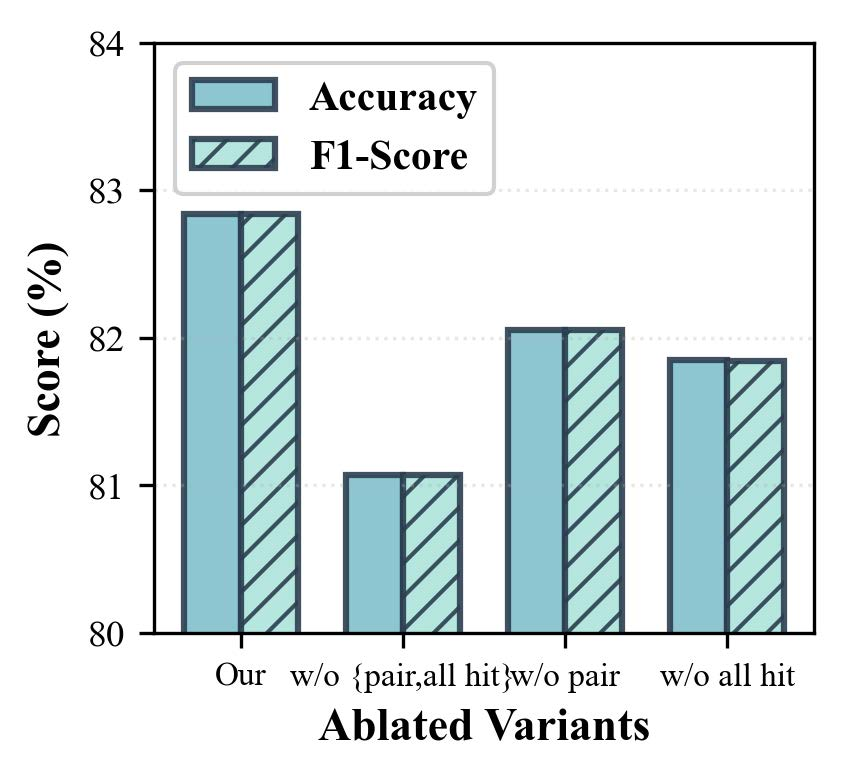
\includegraphics[width=\linewidth]{fig_3a.jpeg}
            \subcaption{PrideMM Performance}
        \end{minipage}
        \hfill
        \begin{minipage}{0.48\linewidth}
            \centering
            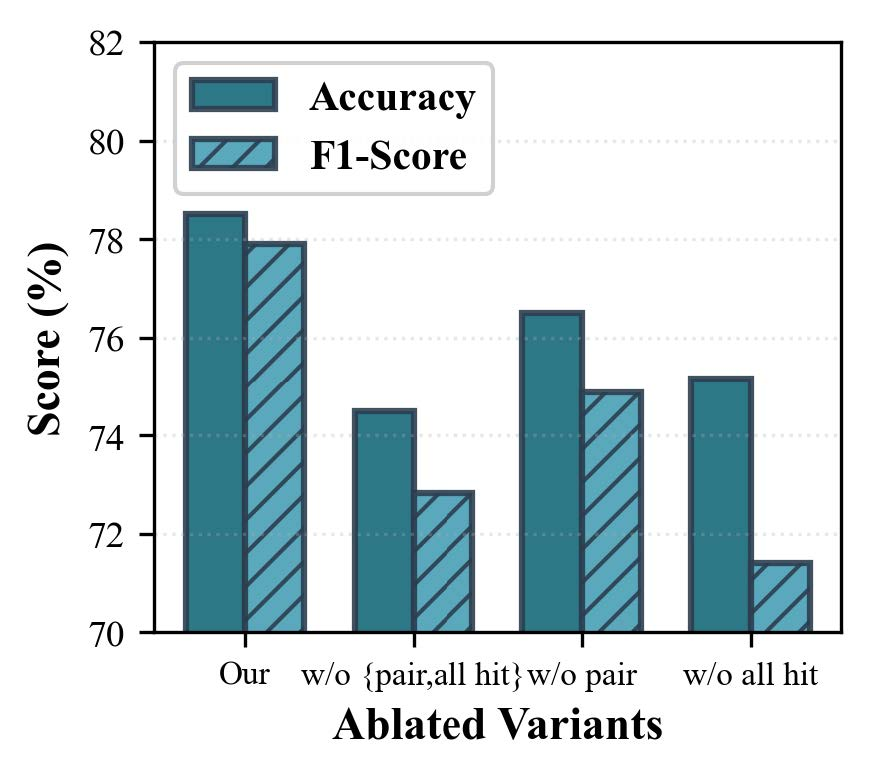
\includegraphics[width=\linewidth]{fig_3b.jpeg}
            \subcaption{MultiOff Performance}
        \end{minipage}
    \end{minipage}
    }
    \caption{Ablation study of the cooperative reward mechanism on PrideMM and MultiOff datasets, reproduced from the original paper.}
    \label{fig:reward-ablation}
\end{figure}

\subsection{Non-game-theoretic Strategies Comparison}

To isolate how much of GECO's improvement actually comes from the game-theoretic
coordination itself (as opposed to simply fine-tuning each LMM better), the authors
compare each of the three individual LMMs when trained normally with supervised
fine-tuning (SFT) against the same models when optimized through GECO instead. These
results are shown in Table~\ref{tab:sft-vs-geco}.

\begin{table}[h]
\centering
\caption{Comparison between supervised fine-tuning (SFT) and GECO across different LMM
backbones on PrideMM and MultiOff (reproduced from the original paper).}
\label{tab:sft-vs-geco}
\begin{tabular}{ll|cc|cc}
\toprule
\textbf{Model} & \textbf{Method} & \multicolumn{2}{c|}{\textbf{PrideMM}} & \multicolumn{2}{c}{\textbf{MultiOff}} \\
 & & Acc & F1 & Acc & F1 \\
\midrule
\multirow{2}{*}{LLaVA} & SFT  & 78.70 & 78.74 & 67.79 & 58.62 \\
                        & GECO & \textbf{81.45} & \textbf{81.64} & \textbf{70.46} & 57.10 \\
\midrule
\multirow{2}{*}{Qwen}  & SFT  & 77.51 & 77.20 & 66.44 & 44.44 \\
                        & GECO & \textbf{78.90} & \textbf{78.90} & \textbf{68.46} & \textbf{44.47} \\
\midrule
\multirow{2}{*}{Gemma} & SFT  & 75.74 & 75.74 & 65.10 & 65.79 \\
                        & GECO & \textbf{77.91} & \textbf{77.78} & \textbf{76.51} & \textbf{71.54} \\
\bottomrule
\end{tabular}
\end{table}

Across almost every metric on both datasets, GECO outperforms directly supervised
fine-tuning of the same backbone model. This suggests that the improvement is not simply
coming from better individual training, but from the strategic coordination the game
introduces -- by encouraging agents to exploit each other's complementary strengths while
still working against their individual biases, GECO produces more consistent and robust
single-model performance than plain SFT alone.

The authors then compare GECO against two other multi-agent ensemble strategies that do
not use game theory: a simple voting-based ensemble, and a debate-based ensemble. These
results are shown in Table~\ref{tab:ensemble-comparison}.

\begin{table}[h]
\centering
\caption{Comparison between GECO and non-game-theoretic ensemble strategies on PrideMM and
MultiOff (reproduced from the original paper).}
\label{tab:ensemble-comparison}
\begin{tabular}{ll|cc|cc}
\toprule
\textbf{Category} & \textbf{Method} & \multicolumn{2}{c|}{\textbf{PrideMM}} & \multicolumn{2}{c}{\textbf{MultiOff}} \\
 & & Acc & F1 & Acc & F1 \\
\midrule
\multirow{2}{*}{Non-Game} & Voting & 79.49 & 79.37 & 69.80 & 59.46 \\
                          & Debate & 79.88 & 79.87 & 73.15 & 70.72 \\
\midrule
Game & \textbf{GECO} & \textbf{82.84} & \textbf{82.84} & \textbf{78.52} & \textbf{77.90} \\
\bottomrule
\end{tabular}
\end{table}

While both ensemble strategies do improve over a single SFT model, they still fall
noticeably short of GECO. The voting-based ensemble treats every agent's vote equally,
which ignores the fact that different models are not equally reliable and may share
overlapping biases. The debate-based ensemble does introduce interaction between agents,
but its final decision still depends heavily on the fairness of the judge model, which can
end up reinforcing bias rather than correcting it. GECO's explicit game-theoretic
formulation, by contrast, drives agents toward adaptive alignment through the reward
structure itself, which the authors argue is why it consistently achieves the highest
accuracy and F1 scores across both datasets.

\subsection{Parameter Analysis}

To understand how sensitive GECO is to the specific reward weights chosen, the authors
run a parameter analysis on both the all-hit bonus $\beta$ and the pairwise hit bonus
$\lambda$, keeping the individual hit bonus $\alpha$ fixed at its default value of 1.0.
The results on both PrideMM and MultiOff are shown in Figure~\ref{fig:param-analysis}.

To isolate the effect of the all-hit bonus $\beta$ first, the pairwise hit bonus $\lambda$
is temporarily set to 0. Across the tested range of $\beta \in [0.9, 1.2]$, GECO's
performance stays fairly stable, which suggests the framework is not particularly
sensitive to the exact value chosen for this term -- it mainly needs to be present at a
reasonable strength rather than tuned precisely.

The authors then fix $\beta$ back to 1.0 and instead vary the pairwise hit bonus
$\lambda$. Here, the behavior is quite different: performance in both accuracy and F1
drops noticeably when $\lambda$ is set too low ($\leq 0.3$) or too high ($\geq 0.9$). This
suggests that the pairwise incentive plays a more delicate balancing role in the reward
scheme -- when it is too weak, agents are not sufficiently encouraged to align with one
another, and effective collaboration breaks down. When it is too strong, however, the
reward starts introducing its own bias into training, increasing the risk of the model
overfitting to spurious agreement between agents rather than genuinely correct
predictions.

\begin{figure}[h]
    \centering
    \resizebox{0.8\linewidth}{!}{%
    \begin{minipage}{\linewidth}
        \centering
        \begin{minipage}{0.48\linewidth}
            \centering
            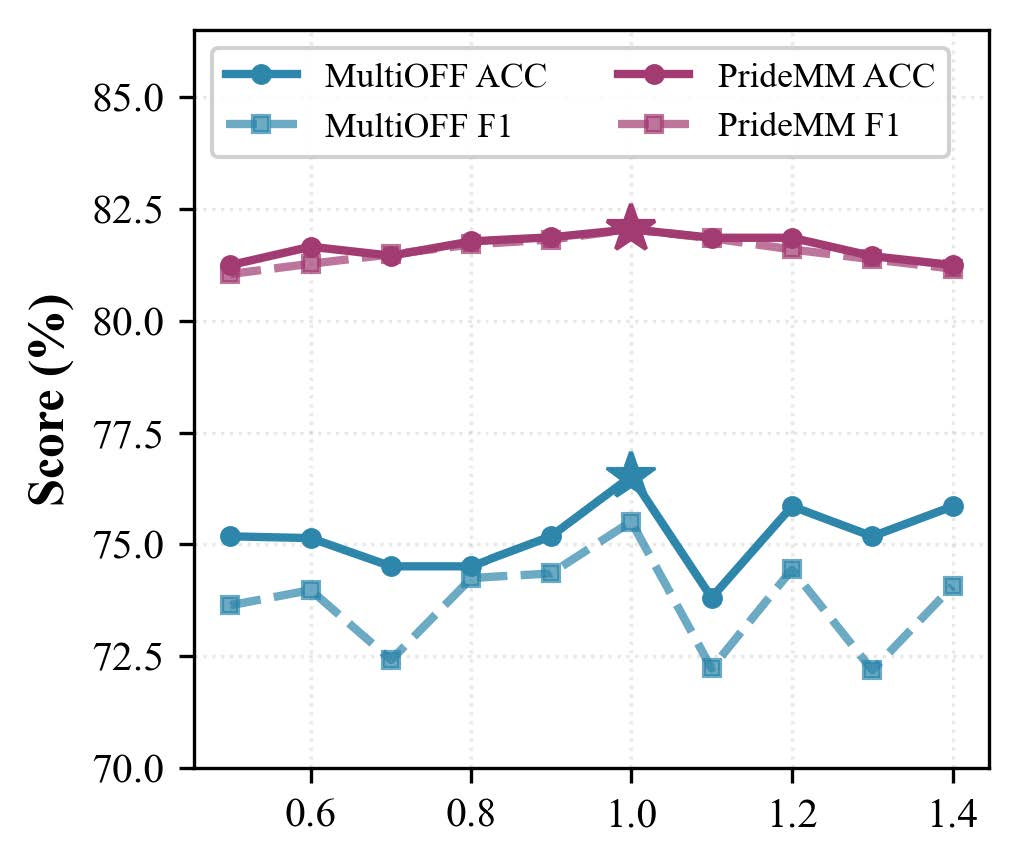
\includegraphics[width=\linewidth]{fig_4a.jpeg}
            \subcaption{All-hit bonus $\beta$}
        \end{minipage}
        \hfill
        \begin{minipage}{0.48\linewidth}
            \centering
            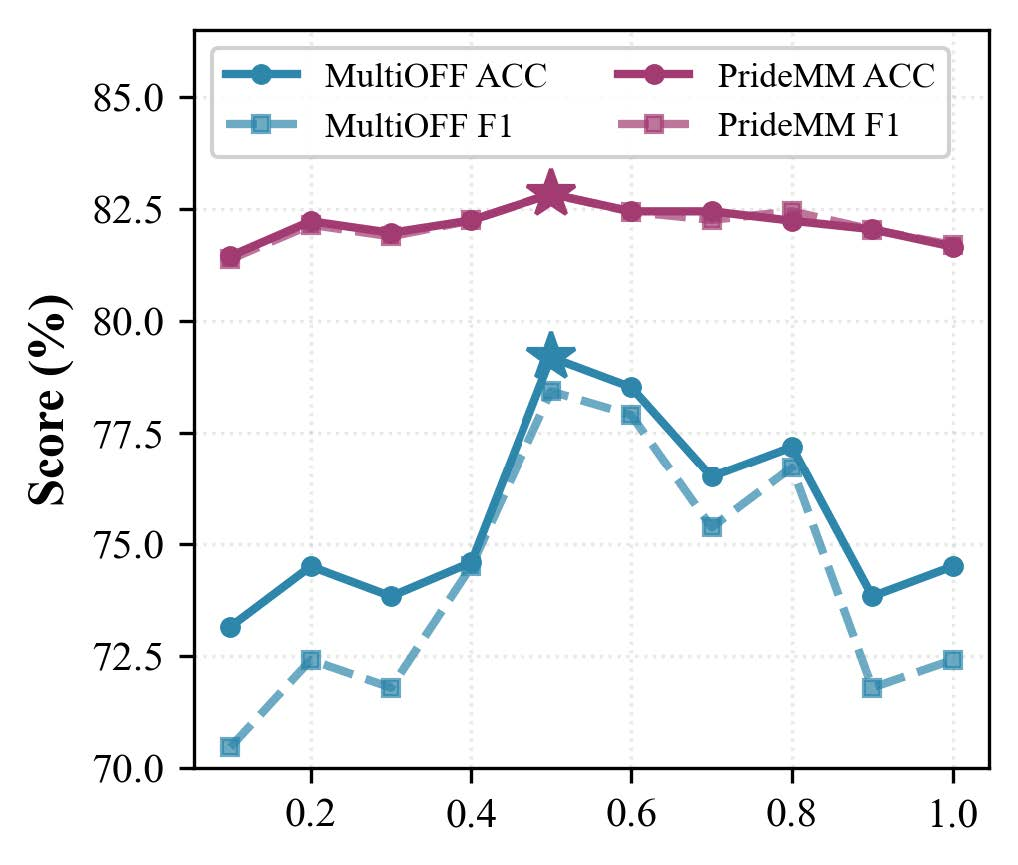
\includegraphics[width=\linewidth]{fig_4b.jpeg}
            \subcaption{Pairwise hit bonus $\lambda$}
        \end{minipage}
    \end{minipage}
    }
    \caption{Parameter analysis of the all-hit bonus $\beta$ and the pairwise hit bonus
    $\lambda$ on PrideMM and MultiOff datasets, reproduced from the original paper.}
    \label{fig:param-analysis}
\end{figure}

\subsection{Case Study}

To make the advantages of GECO more concrete, the authors walk through two qualitative
examples comparing it against voting-based and debate-based methods, shown in
Figure~\ref{fig:case-study}.

In the first example, the reasoning agents disagree on whether a meme is hateful. This
disagreement causes the simple voting-based method to settle on the wrong label, since it
just follows whichever answer the majority happens to pick. The debate-based method also
fails here -- the interaction between agents does not resolve the underlying
disagreement, and the judge model ends up siding with the biased majority, producing an
incorrect decision with very low confidence. GECO, by contrast, uses its cooperative
game-theoretic mechanism to guide all agents toward a jointly optimal strategy that
achieves a higher overall utility. As a result, it correctly classifies the sample with
very high confidence, successfully working through the disagreement that broke the other
two methods.

The second example shows a case where all methods actually arrive at the correct
classification. Even here, though, GECO shows a clear advantage: it reaches its correct
decision with much higher confidence, reflecting a higher overall utility value, whereas
the debate-based method remains comparatively uncertain due to inconsistent reasoning
among its agents. This suggests that GECO's benefit is not limited to cases where other
methods fail outright -- it also produces more reliable, better-calibrated confidence
even when everyone agrees.

\begin{figure}[h]
    \centering
    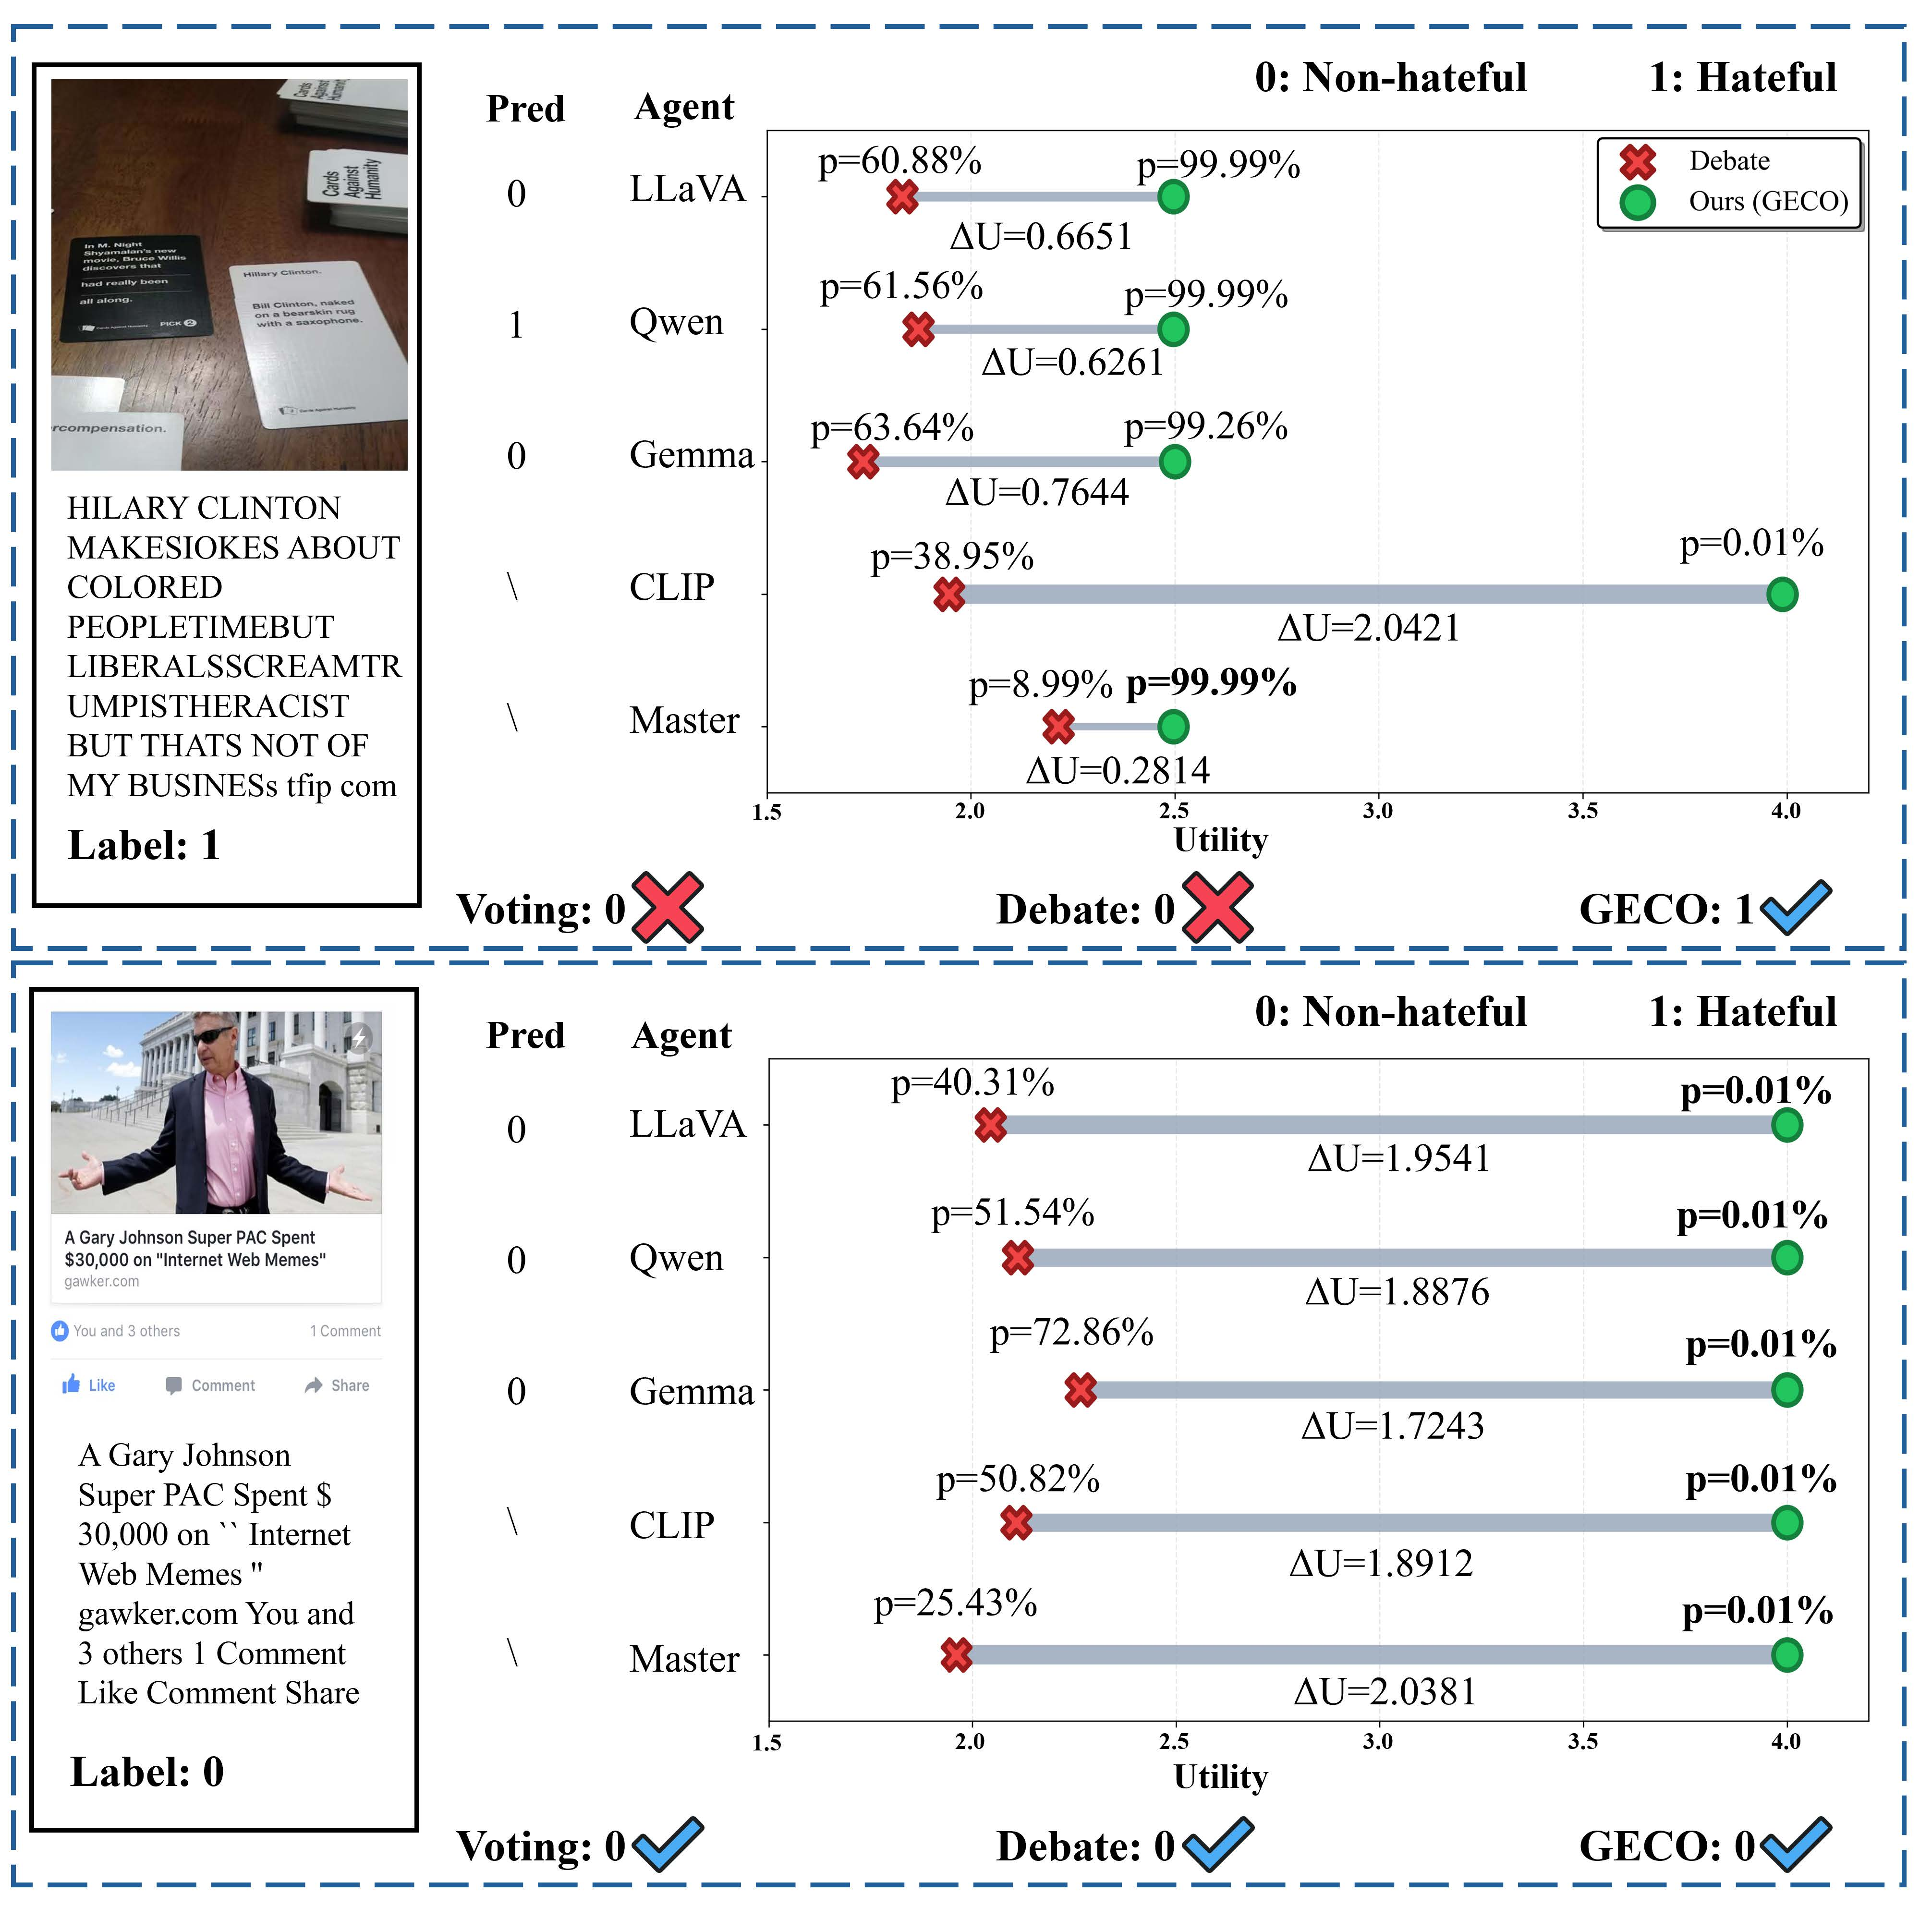
\includegraphics[width=0.7\linewidth]{fig_5.jpeg}
    \caption{Case study illustrating the decision performance of different methods,
    reproduced from the original paper. $\Delta U$ represents the difference in
    conditional expected utility between GECO and the ensemble methods.}
    \label{fig:case-study}
\end{figure}

To dig a little deeper into \emph{why} GECO is able to correct these biased decisions, there is a 
more detailed case in Figure~\ref{fig:visualized-case}. This
example contains lexical cues that mislead every SFT-trained model into incorrectly
labeling the meme as hateful. Once GECO is applied, the system manages to correct this
shared failure and steer most of the agents toward the correct, non-hateful prediction.

The utility values behind this correction reveal the actual mechanism driving the change.
Although Qwen initially sticks with its incorrect prediction, the analysis shows that its
potential utility for switching to the correct action is substantially higher than what it
currently receives -- this gap, driven mainly by the strong incentive from the all-hit
bonus, is what motivates the agent to shift toward the correct decision as training
continues. Agents that have already reached the correct consensus, on the other hand, sit
in a stable equilibrium, where changing their prediction on their own would only lower
their own payoff, so they have no incentive to deviate. Overall, this example illustrates
how the multi-agent system gradually moves from a low-payoff, biased region toward a
higher-payoff region of correct, shared consensus.

\begin{figure}[h]
    \centering
    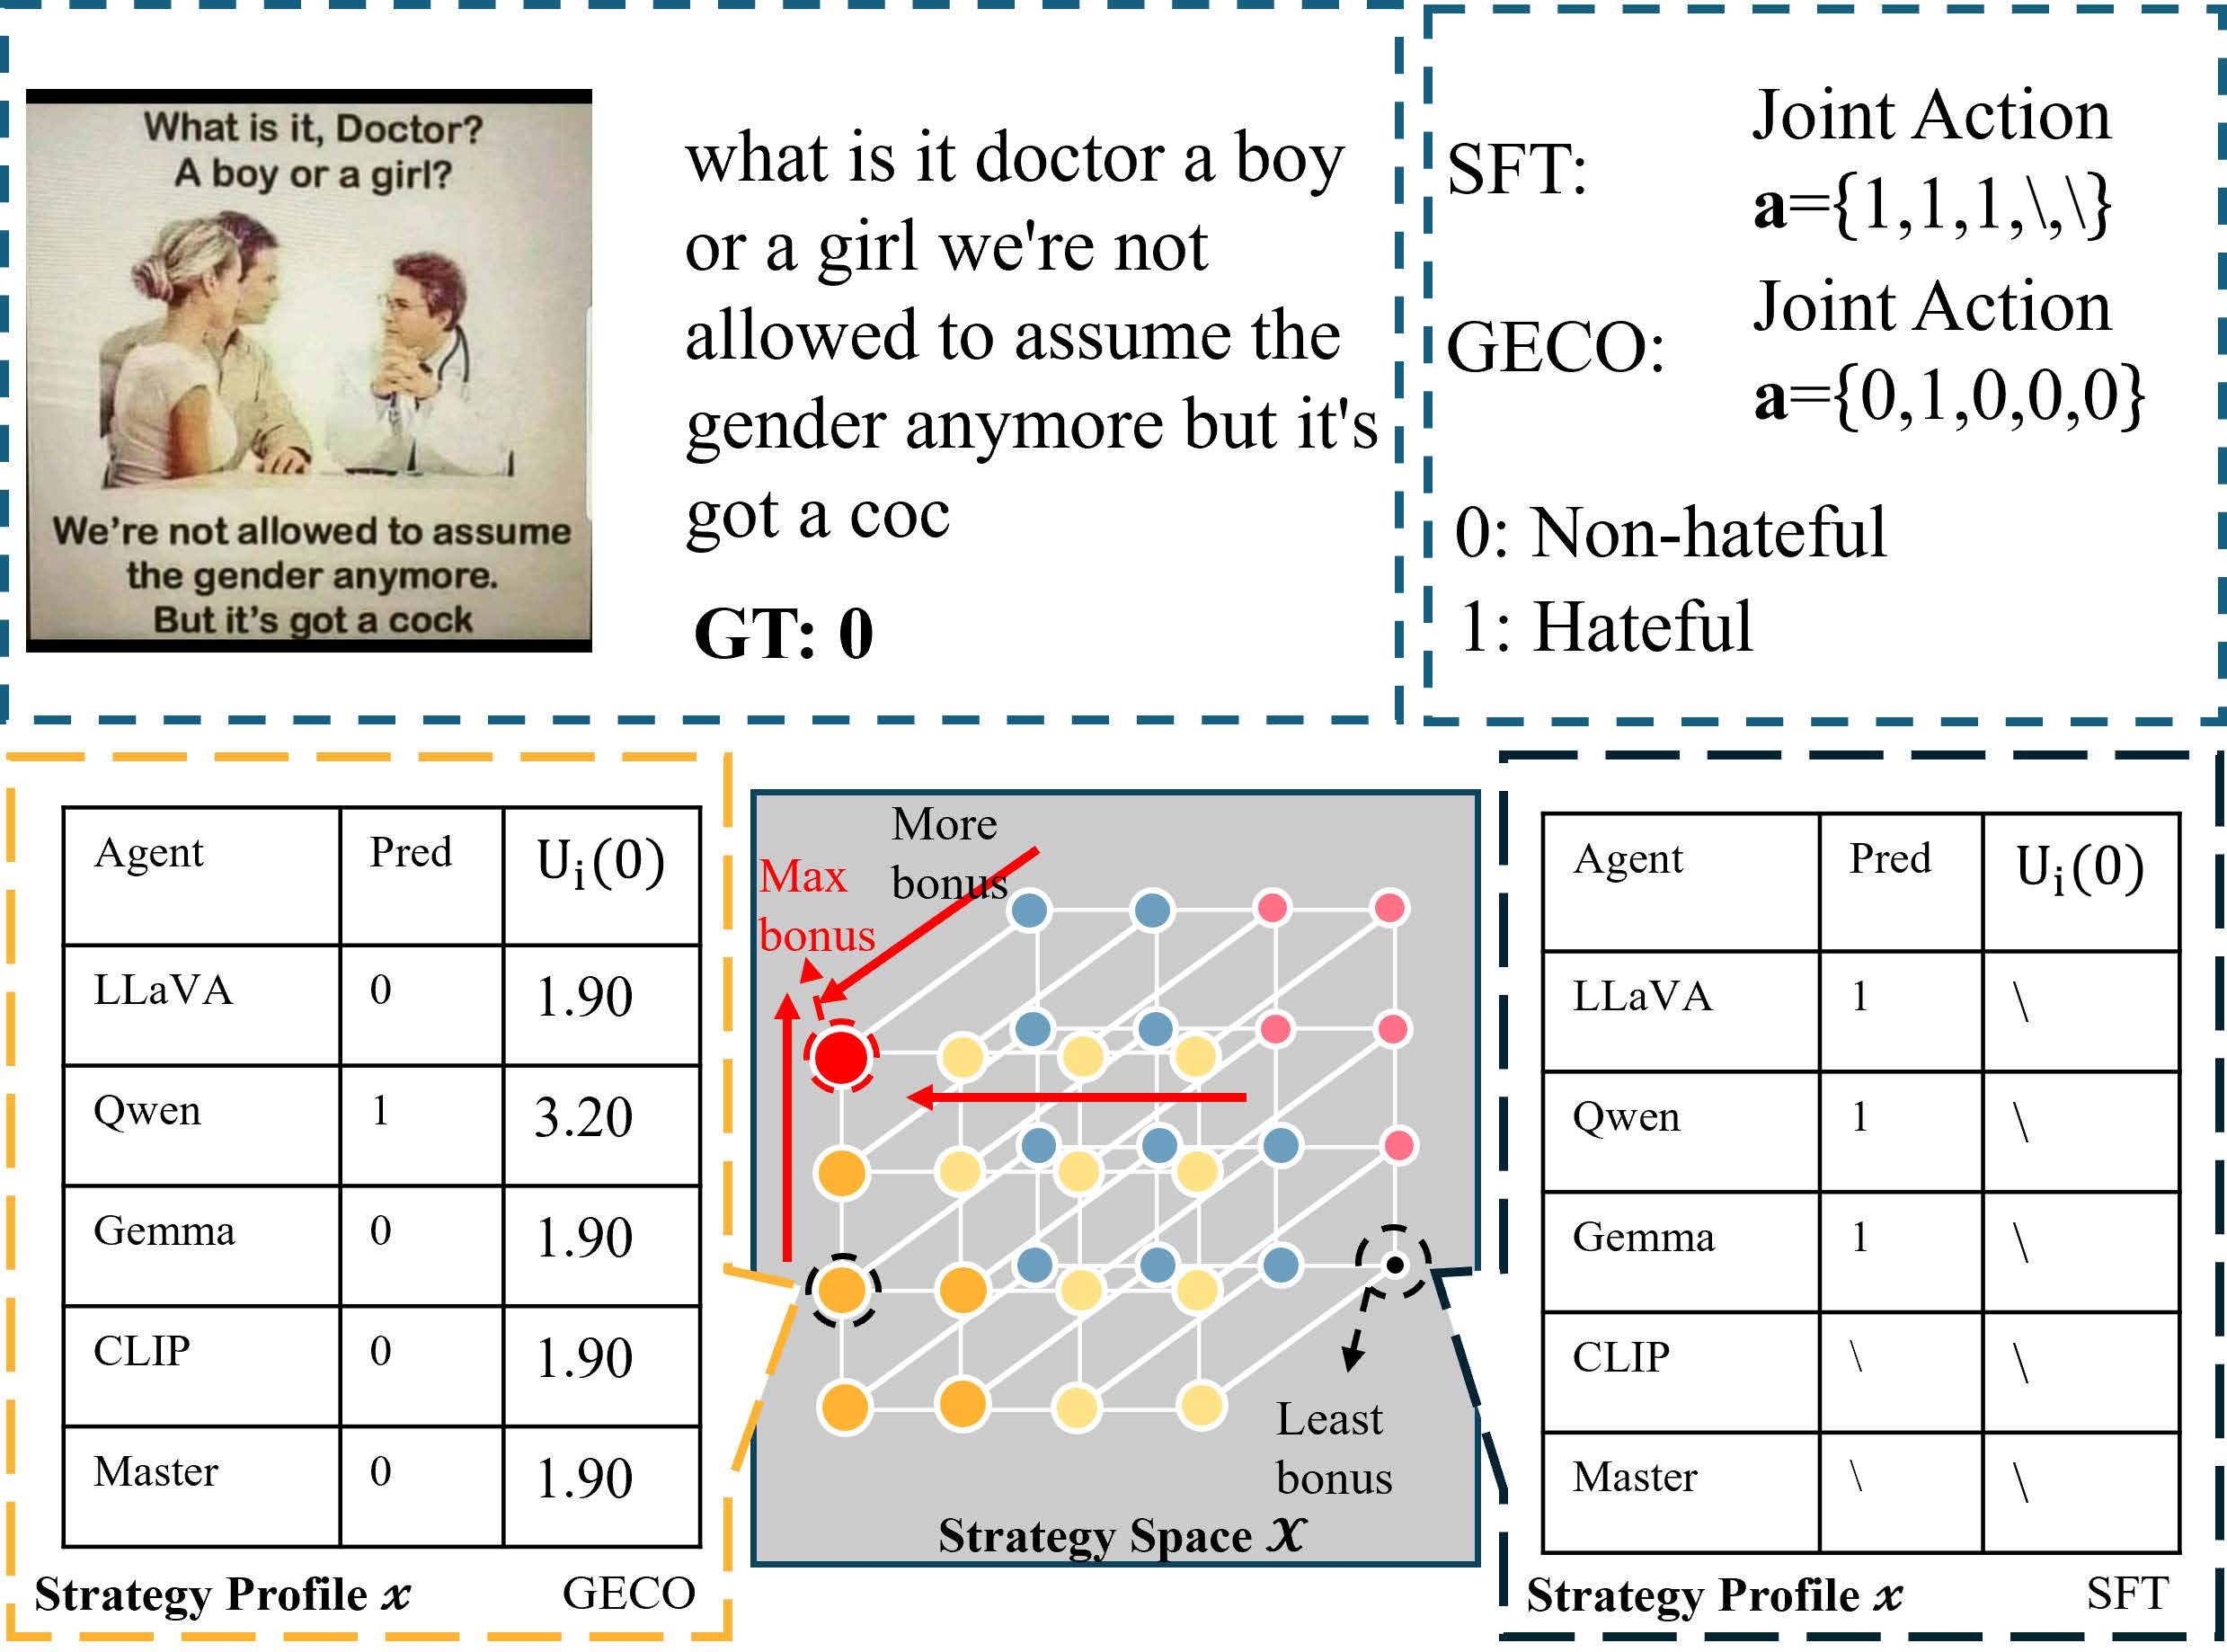
\includegraphics[width=0.7\linewidth]{fig_6.jpeg}
    \caption{Visualized case analysis illustrating how GECO corrects biased collective
    predictions during the decision-making process, reproduced from the original paper.}
    \label{fig:visualized-case}
\end{figure}

\section{Conclusion}

This reproduction summarized GECO, a game-theoretic multi-agent framework proposed for
reducing bias in hateful meme classification. Instead of relying on a single LMM or on
simpler ensembling strategies like voting or debate, GECO frames the collaboration between
multiple heterogeneous LMMs as a cooperative game, using a specifically designed mixed
bonus scheme to push the agents toward mutual agreement on the correct label rather than
just individual correctness. Across five public benchmark datasets, the original paper
reports that GECO consistently surpasses prior state-of-the-art methods, including both
CLIP-based classifiers and more recent LMM-based and debate-based ensembles.
The ablation studies and case studies presented in the paper further support the authors'
central claim: each component of the framework -- the reasoning agents, the learnable
CLIP-based agent, and especially the master agent -- contributes meaningfully to the final
performance, and removing any of them (individually or in pairs) causes a clear drop in
accuracy. The qualitative case studies also make a compelling argument that GECO does not
just improve raw accuracy numbers, but genuinely helps resolve cases where individual
models disagree due to differing biases, which voting- and debate-based methods struggle
to handle reliably.
Overall, reproducing this paper highlighted how combining formal game-theoretic principles
with modern large multimodal models can offer a more principled way to design multi-agent
ensembles, compared to relying on simpler heuristics like majority voting or ad hoc debate
protocols.
\bibliography{references}
\end{document}